
\documentclass{beamer}
\usepackage{amsmath}
\usepackage{graphicx}
\graphicspath{ {./images/} }

\title{Least squares}
\subtitle{Sample Subtitle}
\author{Juan V. Vía}
\institute{}
\date{\today}

%\usetheme{lucid}
\begin{document}
% -------------------------------------------------------------------------
\frame {
	\titlepage
}
% -------------------------------------------------------------------------
\frame {
	\frametitle{Example}
	\framesubtitle{Showing why least squares}
	We have a variable $y$. We know that it's dependent of another variable $x$ in some
	way. But we don't know how, exactly.

	So we go to the field and measure certain points. Those that we can reach. Six of them.
	$$(2,5),(5,5),(7,8),(11,7),(14,9),(18,7)$$

	That is: at $x=2$ we measure $y=5$, at $x=5$ we measure $y=5$ again, but
	at $x=7$ we got $y=8$, and so on.
}
% -------------------------------------------------------------------------
\frame {
	\frametitle{Example}
	\framesubtitle{Showing why least squares}
	Next step, obviously, is to plot these points.
	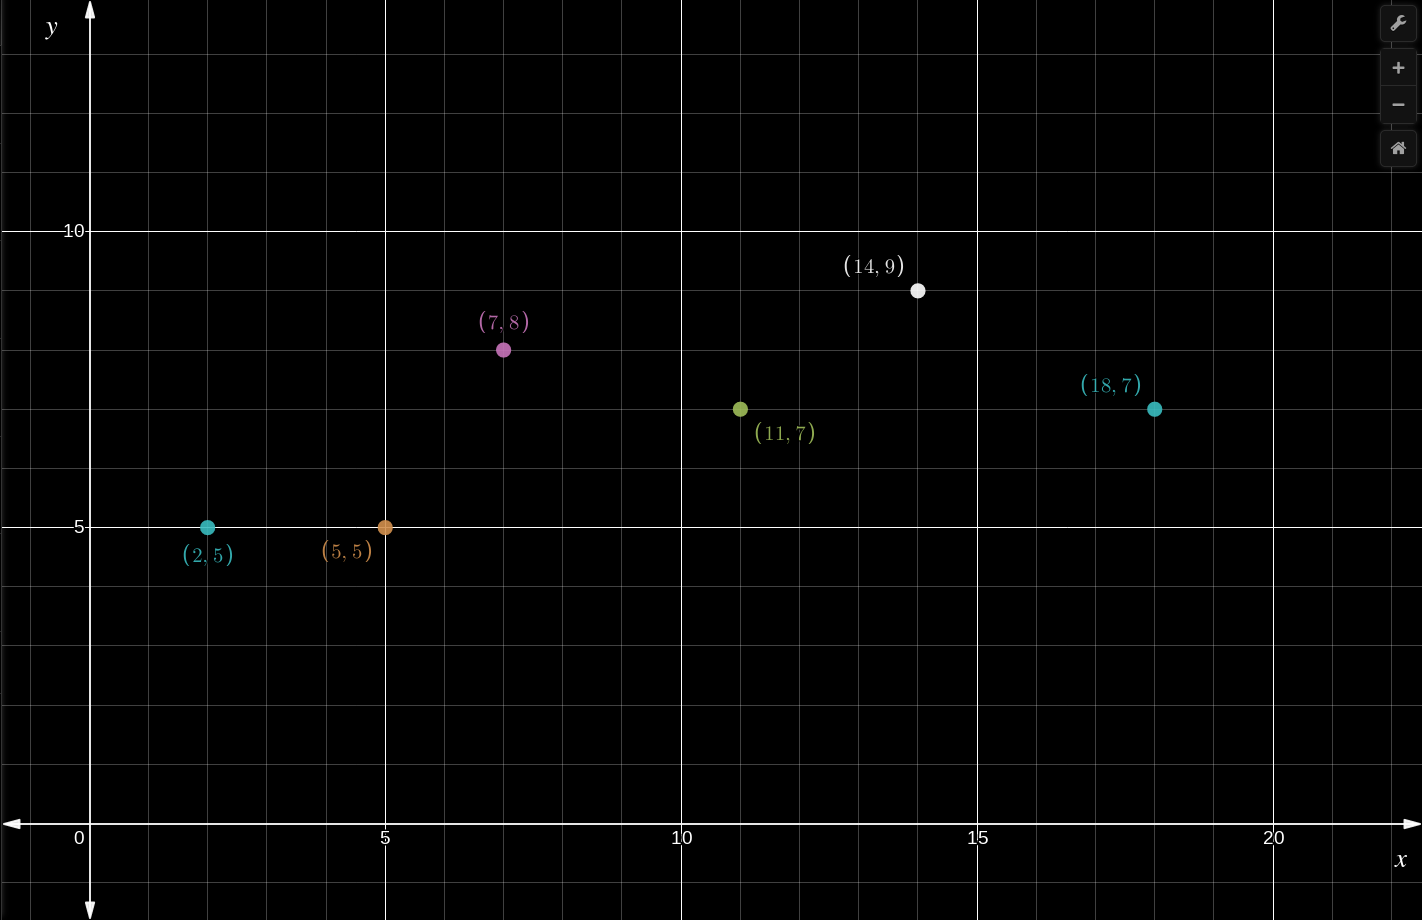
\includegraphics[width=8cm]{points}
}
% -------------------------------------------------------------------------
\frame {
	\frametitle{Example}
	\framesubtitle{Showing why least squares}
	Let's start by tracing a line wich "best fit" that data
	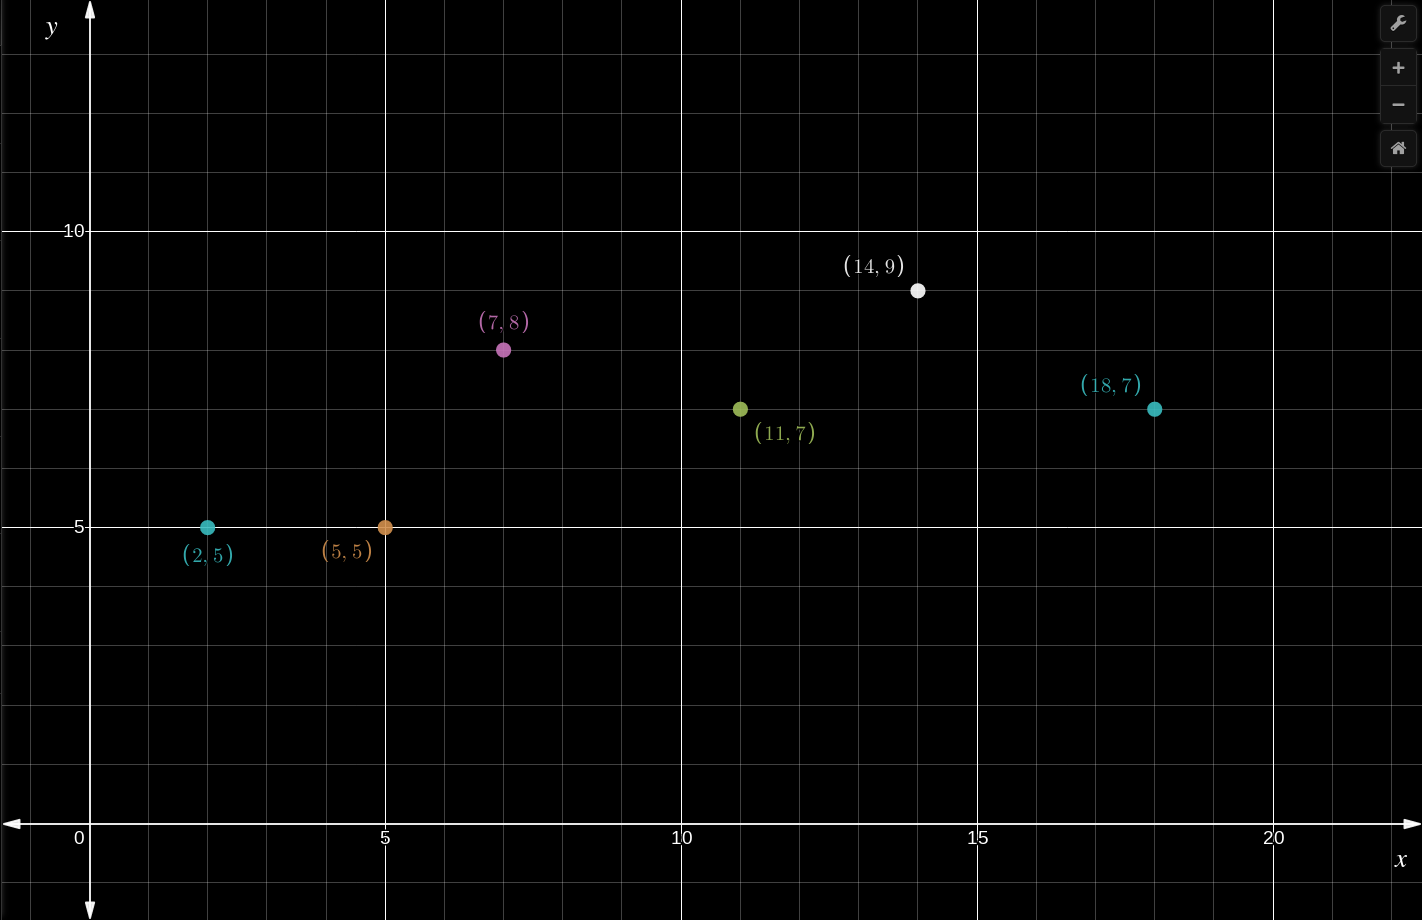
\includegraphics[width=8cm]{points}
}
% -------------------------------------------------------------------------
\frame {
	\frametitle{Example}
	\framesubtitle{Showing why least squares}
	What line? How to choose that line?
	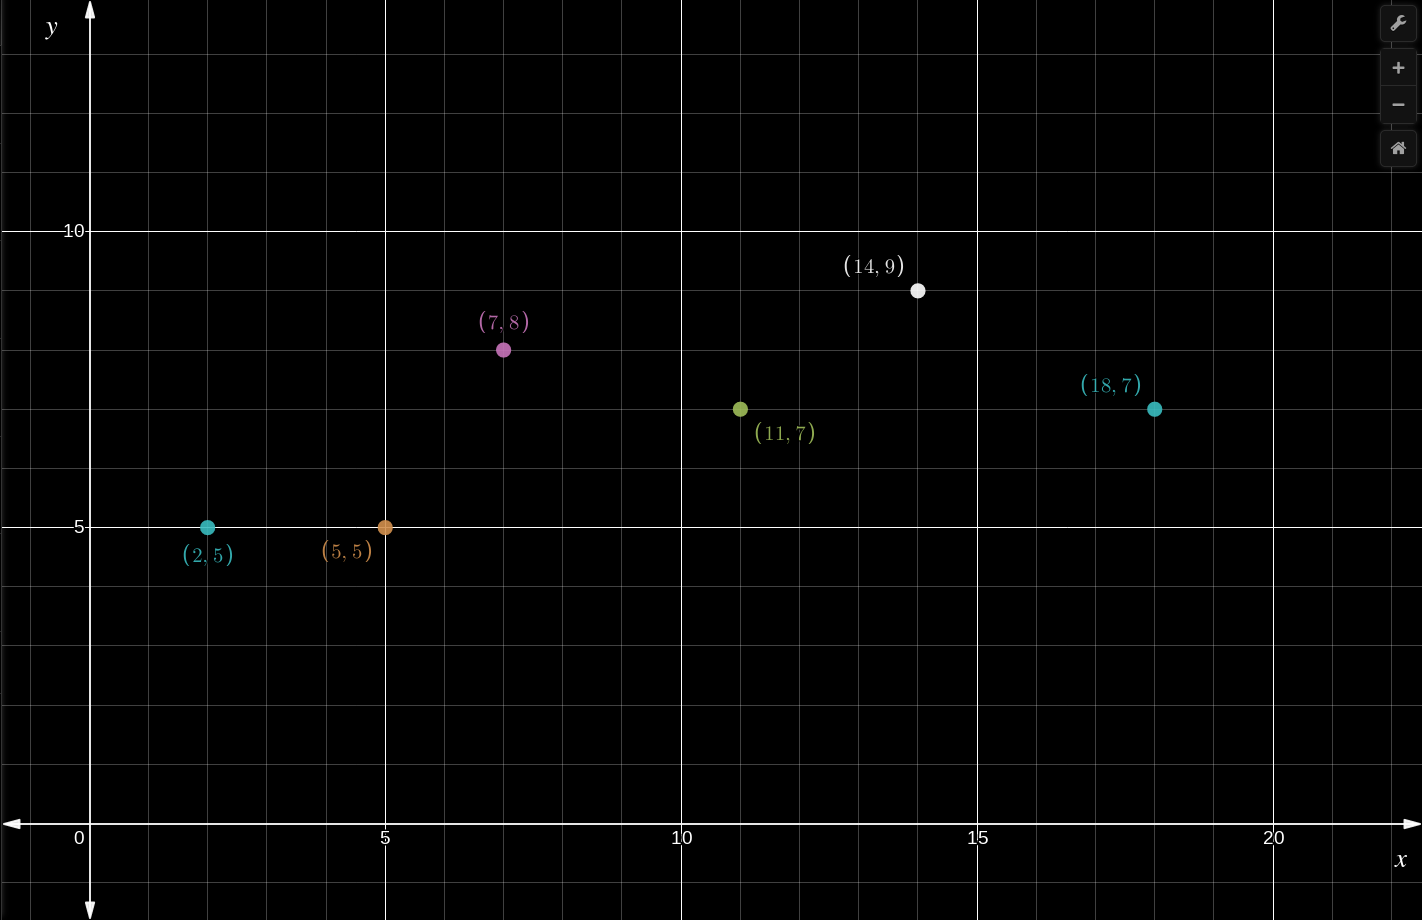
\includegraphics[width=8cm]{points}
}
% -------------------------------------------------------------------------
\frame {
	\frametitle{Example}
	\framesubtitle{Showing why least squares}

	A very common way to express a line is using the equation (a polinomial function)
	$$
		y = mx +b
	$$

	Using vector notation:
	$$y=
		\begin{bmatrix} x & 1 \end{bmatrix}
		\begin{bmatrix} m\\ b \end{bmatrix}$$

	Or, switching terms:
	$$\begin{bmatrix} x & 1 \end{bmatrix}
		\begin{bmatrix} m\\ b \end{bmatrix}=y$$
}
% -------------------------------------------------------------------------
\frame {
	\frametitle{Example}
	\framesubtitle{Showing why least squares}

	Ok. Fine. That's it. This form
	$$\begin{bmatrix} x & 1 \end{bmatrix}
		\begin{bmatrix} m\\ b \end{bmatrix}=y$$
	will be a useful one because we know $x$ and $y$ in six points.
	For example take the first point $(2,5)$
	$$\begin{bmatrix} 2 & 1 \end{bmatrix}
		\begin{bmatrix} m\\ b \end{bmatrix}=5$$
}
% -------------------------------------------------------------------------
\frame {
	\frametitle{Example}
	\framesubtitle{Showing why least squares}

	And yes, your guess is true. We can incorporate the second point $(5,5)$ and get
	$$\begin{bmatrix} 2 & 1 \\
                5 & 1\end{bmatrix}
		\begin{bmatrix} m\\ b \end{bmatrix}=\begin{bmatrix} 5\\ 5 \end{bmatrix}$$

	...and the third point...and the fourth...
}
% -------------------------------------------------------------------------
\frame {
	\frametitle{Example}
	\framesubtitle{Showing why least squares}

	Reaching the end this is the result
	$$\begin{bmatrix} 2  & 1 \\
                5  & 1 \\
                7  & 1 \\
                11 & 1 \\
                14 & 1 \\
                18 & 1
		\end{bmatrix}
		\begin{bmatrix} m\\ b \end{bmatrix}=\begin{bmatrix}
			5 \\
			5 \\
			8 \\
			7 \\
			9 \\
			7
		\end{bmatrix}$$
}
% -------------------------------------------------------------------------
\frame {
	\frametitle{Example}
	\framesubtitle{Showing why least squares}

	Time to name things.

}
% -------------------------------------------------------------------------
\frame {
	\frametitle{Example}
	\framesubtitle{Showing why least squares}

	Call $A$ to the matrix 	$$A=\begin{bmatrix}
			2  & 1 \\
			5  & 1 \\
			7  & 1 \\
			11 & 1 \\
			14 & 1 \\
			18 & 1
		\end{bmatrix}$$
}
% -------------------------------------------------------------------------
\frame {
	\frametitle{Example}
	\framesubtitle{Showing why least squares}

	Call $x$ to the column vector	$$x=\begin{bmatrix} m\\ b \end{bmatrix}$$
}
% -------------------------------------------------------------------------
\frame {
	\frametitle{Example}
	\framesubtitle{Showing why least squares}

	Call $b$ to the column vector	$$b=\begin{bmatrix}
			5 \\
			5 \\
			8 \\
			7 \\
			9 \\
			7
		\end{bmatrix}$$
}
% -------------------------------------------------------------------------
\frame {
	\frametitle{Example}
	\framesubtitle{Showing why least squares}

	Thus, the equation
	$$\begin{bmatrix} 2  & 1 \\
		5  & 1 \\
		7  & 1 \\
		11 & 1 \\
		14 & 1 \\
		18 & 1
\end{bmatrix}
\begin{bmatrix} m\\ b \end{bmatrix}=\begin{bmatrix}
5 \\
5 \\
8 \\
7 \\
9 \\
7
\end{bmatrix}$$
becomes
$$ Ax=b $$
}
% -------------------------------------------------------------------------
\frame {
	\frametitle{Example}
	\framesubtitle{Showing why least squares}
	
}
% -------------------------------------------------------------------------
\end{document}